\Chapter{Fejlesztői dokumentáció}
\label{Chap:dokumen}

\iffalse
Ebben a fejezetben kell a hallgatónak leírnia a saját eredményeit. Például ilyennek tekinthető a hallgató által elkészített program leírása, algoritmus leírása alkalmazási lehetőségek, eredmények. Lehet benne több alfejezet vagy al-alfejezet is. Ezek számozása és a tartalomjegyzékben  való megjelenítése rögzített. A fejezet címe megváltoztatható az eredmények szerint. Ez a fejezet és a \aref{Chap:tema} együtt összesen 25-60 oldal terjedelmű kell hogy legyen
\fi

Az Elméleti kifejtés során meghatározott célokat különböző gépi tanulási módszerekkel lehet megoldani amik eltérő eredménnyel, pontossággal fognak működni. A nehézségi osztályok meghatározására elsősorban a  \myaref{ssec:klaszterezes} pontban részletezett klaszterezési módszerek használhatóak

\Section{Adathalmaz előkészítés}
A fejlesztés legelső lépése az összegyűjtött adatok megfelelő struktúrára való átalakítása és megtisztítása, ezzel megkönnyítve a későbbi feldolgozást valamint növelve a gépi tanulási algoritmusok pontosságát

\SubSection{Adatstruktúra kialakítása}
Az adatgyűjtés elsődleges eszközeként a szakdolgozat keretein belül készített weboldal szolgált, amely minden információt egy JSON alapú adatbázisban tárolt le. Az adathalmaz előkészítésének a legelső lépése a JSON struktúráról való áttérés egy, a Python programozási nyelv által kezelt, könnyen használható adatstruktúrára. Erre a szakdolgozat során a Pandas \cite{python-pandas} nevű Python csomag által megvalósított DataFrame nevű struktúra fog szolgálni , amely segítségével az adatokat táblázathoz hasonló formában lehet tárolni. Egy DataFrame oszlopai egyedi, a fejlesztő által definiált oszlopnevekkel érhetőek el, soraira index használatával lehet hivatkozni. Az oszlopok egyenként különböző típusúak lehetnek és tartalmazhatnak NULL értékeket. A DataFrame egyik legnagyobb előnye az oszlopok nevesítése, amivel könnyen nyomon követhető hogy az aktuális értékek melyik feature-nek felelnek meg, mit reprezentálnak a valóságban

\begin{programreszlet}
A  parancs segítségével a JSON struktúra (jsonData) könnyen átalakítható DataFrame-é (dataset). A dataset oszlopai megfelelnek a \myaref{ssec:adatstruktura} pontban részletezett adatoknak.
\begin{python}
import pandas

jsonData = pandas.read_json("2019_03_20_10h.json", type='series')
cleanData = []
for u in userData:
  if userData[u]['connectedToStrava'] == True:
    for i in range(0,len(userData[user]['activities'])):
       userData[u]['activities'][i]['ageGroup'] = userData[u]['ageGroup']
       userData[u]['activities'][i]['sex'] = userData[u]['sex']
       userData[u]['activities'][i].pop('external_id', None)
       userData[u]['activities'][i].pop('map_id', None)
       userData[u]['activities'][i].pop('map_resource', None)
       userData[u]['activities'][i].pop('map_summary', None)
       cleanData.append(userData[u]['activities'][i]) 
  else:
    print('User does not have any activities')
dataset = pandas.DataFrame(cleanData)

\end{python}
\end{programreszlet}


A fenti parancs segítségével a JSON struktúra (jsonData) könnyen átalakítható DataFrame-é (dataset). A dataset oszlopai megfelelnek a \myaref{ssec:adatstruktura} pontban részletezett adatoknak.


\SubSection{Adattisztítás}
A megfelelő adatstruktúra kialakítása után a következő lépés az adatok megtisztítása. Ez a lépés azért szükséges mert a legfigyelmesebben gyűjtött adathalmaz is tartalmazhat rossz értékeket illetve előfordulhat hogy több helyen hiányzik a valódi érték. Ezeknek a hibáknak a megtalálása és kijavítása több fázisból áll.

%\csvautotabular{adat/rawDataDescription.csv}
A megtaláláshoz első lépés az adatok áttekintése: NULL értékek vizsgálata, egyes jellemzők eloszlásának megtekintése, minimum, maximum és a kvantilisek összehasonlítása. Ehhez nyújt segítséget a \myref{tab:rawDataDescription} táblázat amely a numerikus oszlopokról készült általános jellemzést összegzi. 
\begin{table}[!h]
	\resizebox{\textwidth}{!}{%
		\begin{tabular}{l|l|l|l|l|l|l|l|l|}
			\cline{2-9}
			& \multicolumn{1}{c|}{\textbf{Count}} & \multicolumn{1}{c|}{\textbf{Mean}} & \multicolumn{1}{c|}{\textbf{STD}} & \multicolumn{1}{c|}{\textbf{Min}} & \multicolumn{1}{c|}{\textbf{0.25}} & \multicolumn{1}{c|}{\textbf{0.50}} & \multicolumn{1}{c|}{\textbf{0.75}} & \multicolumn{1}{c|}{\textbf{Max}} \\ \hline
			\multicolumn{1}{|l|}{
				\textbf{age\_group}}  & 10014  & 1.01   & 0.48   & 0.0   & 1.0   & 1.0   & 1.0   & 2.0   \\ \hline
			\multicolumn{1}{|l|}{
				\textbf{average\_speed}}  & 10014   & 24.25   & 653.31  & 0.0  & 4.96   & 5.73  & 6.47  & 36100.0  \\ \hline
			\multicolumn{1}{|l|}{
				\textbf{average\_watts}}  & 1848  & 163.0  & 49.51  & 0.0  & 139.10  & 161.85  & 180.85 & 482.6 \\ \hline
			\multicolumn{1}{|l|}{
				\textbf{distance}} & 10014  & 26153.09 & 29465.23 & 0.0   & 7444.83 & 13751.25 & 34587.2  & 436806.0  \\ \hline
			\multicolumn{1}{|l|}{
				\textbf{elapsed\_time}} & 10014 & 5845.88 & 19296.2  & 0.0  & 1648.00  & 3020.0  & 7343.0  & 1806211.0  \\ \hline
			\multicolumn{1}{|l|}{
				\textbf{elev\_high}} & 9845 & 282.1 & 272.66 & -71.2  & 162.2  & 229.4  & 296.4 & 12103.0  \\ \hline
			\multicolumn{1}{|l|}{
				\textbf{elev\_low}}  & 9844  & 131.99 & 68.68  & -500.0  & 103.1 & 130.0 & 148.3  & 1484.0 \\ \hline
			\multicolumn{1}{|l|}{
				\textbf{kilojoules}} & 1765 & 1295.76 & 756.06 & 0.0 & 728.7 & 1236.7 & 1745.4  & 5928.8   \\ \hline
			\multicolumn{1}{|l|}{
				\textbf{max\_speed}} & 10014  & 12.14 & 3.99  & 0.0  & 9.6 & 11.6  & 14.48  & 122.7        \\ \hline
			\multicolumn{1}{|l|}{
				\textbf{max\_watts}} & 546 & 630.95  & 244.34  & 115.0 & 502.0 & 603.0  & 708.0 & 2428.0   \\ \hline
			\multicolumn{1}{|l|}{
				\textbf{moving\_time}}  & 10014  & 4543.18  & 5016.52  & 0.0 & 1442.0  & 2451.0  & 6109.0  & 90983.0  \\ \hline
			\multicolumn{1}{|l|}{
				\textbf{pr\_count}}  & 1959  & 1.48  & 3.2 & 0.0 & 0.0 & 0.0  & 2.0   & 50.0       \\ \hline
			\multicolumn{1}{|l|}{
				\textbf{resource\_state}}  & 1959  & 2.0  & 0.0  & 2.0  & 2.0  & 2.0  & 2.0  & 2.0                \\ \hline
			\multicolumn{1}{|l|}{
				\textbf{\begin{tabular}[c]{@{}l@{}}total\_elevation\\ \_gain\end{tabular}}}  & 10014  & 278.7  & 428.88  & 0.0  & 27.5   & 85.2 & 361.8   & 4416.8   \\ \hline
			\multicolumn{1}{|l|}{
				\textbf{\begin{tabular}[c]{@{}l@{}}weighted\_average\\ \_watts\end{tabular}}} & 546  & 188.86  & 30.35  & 5.0   & 176.25  & 195.0  & 208.75  & 246.0  \\ \hline
			\multicolumn{1}{|l|}{
				\textbf{workout\_type}}  & 4039    & 9.74   & 1.85   & 0.0  & 10.0  & 10.0  & 10.0    & 12.0 \\ \hline
		\end{tabular}%
	}
\caption{Nyers adathalmaz numerikus oszlopainak leírása}
\label{tab:rawDataDescription}
\end{table}

A táblázat oszlopainak a jelentése:
\begin{itemize}
	\item Count: adott jellemző nem NULL értékeinek darabszámát adja meg
	\item Mean: adott jellemző átlaga
	\item STD (Standard Deviation): adott jellemző szórása
\end{itemize}

Sok gond már a táblázat alapján is felfedezhető: sok jellemző tartalmaz NULL értékeket  (average\_watts, kilojoules stb.), máshol pedig olyan értékek szerepelnek amelyek érvénytelenek, értelmezhetetlenek az adott jellemzőre nézve (pl.: distance legkisebb értéke 0 méter; average\_speed legnagyobb értéke 36100 m/s (129960 km/h)). Az ehhez hasonló hibás adatok megtalálása és valamilyen jellegű javítása kritikus feladat, részletezésük a továbbiakban található.


\subsubsection{NULL értékek}
Egy általános adatbázis esetén gyakran előfordul hogy egyes oszlopok NULL értékeket tartalmaznak - ebben az esetben például NULL jelöli ha egy útvonal nincs elérhető adat egy adott jellemzőről. Azonban a gépi tanulási algoritmusok számokat képesek feldolgozni így elengedhetetlen a NULL értékek kiküszöbölése valamilyen formában.

A NULL értékek kiküszöbölésére két elterjedt megoldás létezik:
\begin{itemize}
	\item \textbf{NULL értékek törlése:} az egyszerűbb megoldás a NULL értékeket tartalmazó sorok törlése, azonban ennek a módszernek nagy hátránya hogy sok NULL-t tartalmazó adathalmaz esetén jelentős mértékben megcsappan az adathalmaz mérete
	\item \textbf{NULL értékek feltöltése:} összetettebb, azonban sok esetben célravezetőbb megoldást jelent a NULL értékek helyettesítése valamilyen számított értékkel. Az új értékek számítása különböző módokon történhet, ez nagyban függ az adott jellemző jellegétől
\end{itemize}
Amennyiben egy oszlop nagy mértékben tartalmaz NULL értékeket érdemes megfontolni az elvetését vagy külön esetként kezelni mikor van tényleges érték

Az adat vizsgálata után az első szembetűnő gond a hiányzó értékek. Az alábbi jellemzők akkora mértékben hiányosak hogy a javításuk reménytelen feladat, így az adattisztítás elején törlésre kerültek.
\begin{itemize}
	\item average\_watts: 18.45\% hasznos értéket tartalmaz
	\item commute: 98.83\% hasznos értéket tartalmaz azonban ezekből csupán 23 Igaz érték tehát valójában kevesebb mint 1.0\% használható 
	\item device\_watts : 19.56\% hasznos értéket tartalmaz
	\item flagged : 19.56\% hasznos értéket tartalmaz
	\item has\_heartrate : 19.56\% hasznos értéket tartalmaz
	\item heartrate\_opt\_out: \TODO hasznos értéket tartalmaz
	\item kilojoules : 17.63\% hasznos értéket tartalmaz
	\item max\_watts 5.54\% hasznos értéket tartalmaz
	\item pr\_count : 19.56\% hasznos értéket tartalmaz
	\item resource\_state : 19.56\% hasznos értéket tartalmaz
	\item weighted\_average\_watts : 5.45\% hasznos értéket tartalmaz
	\item sex : 100\% hasznos azonban elenyészően kevés női adatot tartalmaz az adathalmaz, ezért a torzítatlanság érdekében a szakdolgozat során csak a férfi útvonalak kerülnek felhasználásra - így ez az jellemző funkcióját veszti, konstans érték
	\item start\_latlng : 18.34\%
	\item end\_latlng : 18.34\%
\end{itemize}


\subsubsection{Kiugró értékek}
Gyakori jelenség hogy egy jellemző tartalmaz néhány magasan kiugró értéket, amelyek sokszor érvényesek azonban fakadhatnak mérési / rögzítési hibából is. Akár érvényes értékek, akár valamilyen hibából erednek érdemes kiküszöbölni őket mivel könnyen eltorzíthatják az eredményeket. 

A kiugró értékek megtalálása egy alapvető módszer került felhasználásra a szakdolgozat készítése során. A kiugró értékeket jellemzőként külön vizsgáljuk. $F$ jellemzőre $x \in F$ érték kiugrónak tekinthető amennyiben

\[  \frac{x - \overline{F}}{\sigma} > 2.5\]
teljesül, ahol $\overline{F}$ az $F$ jellemző átlaga, $\sigma$ pedig $F$ szórása.

Az alábbiakban a különböző jellemzők kiugró érték vizsgálatának részletes leírása található.\\[6pt]

\textbf{Átlagsebesség (average\_speed):}
ez a jellemző m/s-al adja meg az útvonal átlagsebességét. A fenti módszer 10 kiugró értéket talált amik 2182 m/s (7855.2 km/h) és 28290 ms/s (101844.0 km/h) közé esnek. Ekkora sebesség elérése nyilvánvalóan lehetetlen kerékpárral, eredetük az adatsorok megvizsgálása után leszűkíthető a mozgási idő (moving\_time) jellemző mérésének a hiányára / hibájára. Az átlagsebesség számítása ugyanis a távolság és a mozgási idő hányadosaként kerül kiszámításra és a vizsgált kiugró értékeknél a mozgási idő mindenhol 1 másodperc míg a távolság 10 km fölött van. Ezen adatok javítása nem tűnik megvalósíthatónak. Eldobásuk után az adathalmaz 10004 utat tartalmaz.\\[6pt]

\textbf{Távolság (distance):}
a distance jellemző méterben megadva tárolja az egy-egy útvonal során megtett távolságot. Kiugró érték vizsgálat során 313 értéket talált a módszer, amik között a legkisebb érték 99915.1 méter azaz közel 100 km. Ezek az adatsorok azonban minden más szempontból helyes értékeket tartalmaznak és valójában a 100 km-s utak sem lehetetlenek. Ezek az értékek nem kerültek törlésre az adathalmazból azonban a későbbiek során érdemes lehet a hasonlóan hosszú utakat külön kezelni.\\[6pt]

\textbf{Legmagasabb tengerszint feletti pont (elev\_high):}
az elev\_high jellemző vizsgálata során 61 kiugró érték jelzett a módszer amelyek 976.6 méter és 12103.0 méter közé esnek. A 12103 méter egyértelműen lehetetlen, a többi érték pedig vele együtt elvetésre kerül. Ezen adatsorok eldobása után az adathalmaz 9943 útvonalat tartalmaz.\\[6pt]

\textbf{Legnagyobb sebesség (max\_speed)}
a max\_speed az útvonal során mért maximális sebességet jelzi m/s mértékegységben. Vizsgálata során a használt módszer 218 kiugró értéket talált. Ezek az értékek két intervallumra oszthatóak fel. 0.0 m/s - 2.1 m/s és 22.1 m/s - 122.7 ms azaz 0.0 km/h - 7.56 km/h és 79.56 km/h - 441.72 km/h. Ezek olyan adatok amelyek kilógnak az adathalmazból, sok közülük lehetetlen / értelmezhetetlen. Ezen adatsorok eldobása után az adathalmaz 9725 útvonalat tartalmaz.\\[6pt]

\textbf{Mozgási idő (moving\_time)}
a moving\_time jellemző a tényleges mozgással töltött időt tárolja másodpercben megadva. A jellemző vizsgálata során 276 érték bizonyult kiugrónak amelyek közül a legkisebb értéke 16814 másodperc azaz nagyjából 4 óra és 40 perc. Ezek az értékek összefüggnek a távolság (distance) jellemző vizsgálata során talált kiugró értékekkel, így egyenlőre az adathalmaz része marad, a későbbiek során azonban külön lesz kezelve.


A kiugró értékek megtalálására használt módszeren felül definiálásra került néhány szabály amik segítségével ki lehet szűrni az egyéb helytelen adatokat. Ezek alapján elvetésre kerülnek azok az adatsorok ahol:
\begin{itemize}
	\item az átlagsebesség kisebb mint 2 m/s (7.2 km/h)
	\item a távolság kisebb mint 100 méter (néhány száz méter esetén előfordulhat hogy rövid sprinteket tettek meg a sportolók)
	\item a legmagasabb vagy legalacsonyabb tengerszint feletti magasság hiányzó adat
\end{itemize} 
Továbbá 2 helyen javításra került az összes eltelt idő (elapsed\_time) mivel kevesebb volt mint a mozgással tölött idő (moving\_time)


A fentebbi adatsorok eldobása után összességében 9603 útvonalat tartalmazó adathalmaz maradt.


\SubSection{Adatok áttekintése}
A további feldolgozás illetve a tényleges gépi tanulási algoritmusok felhasználása előtt érdemes kicsit mélyrehatóbban tanulmányozni az adathalmazt, felfedezni a mintákat és összefüggéseket. 



\begin{figure}
	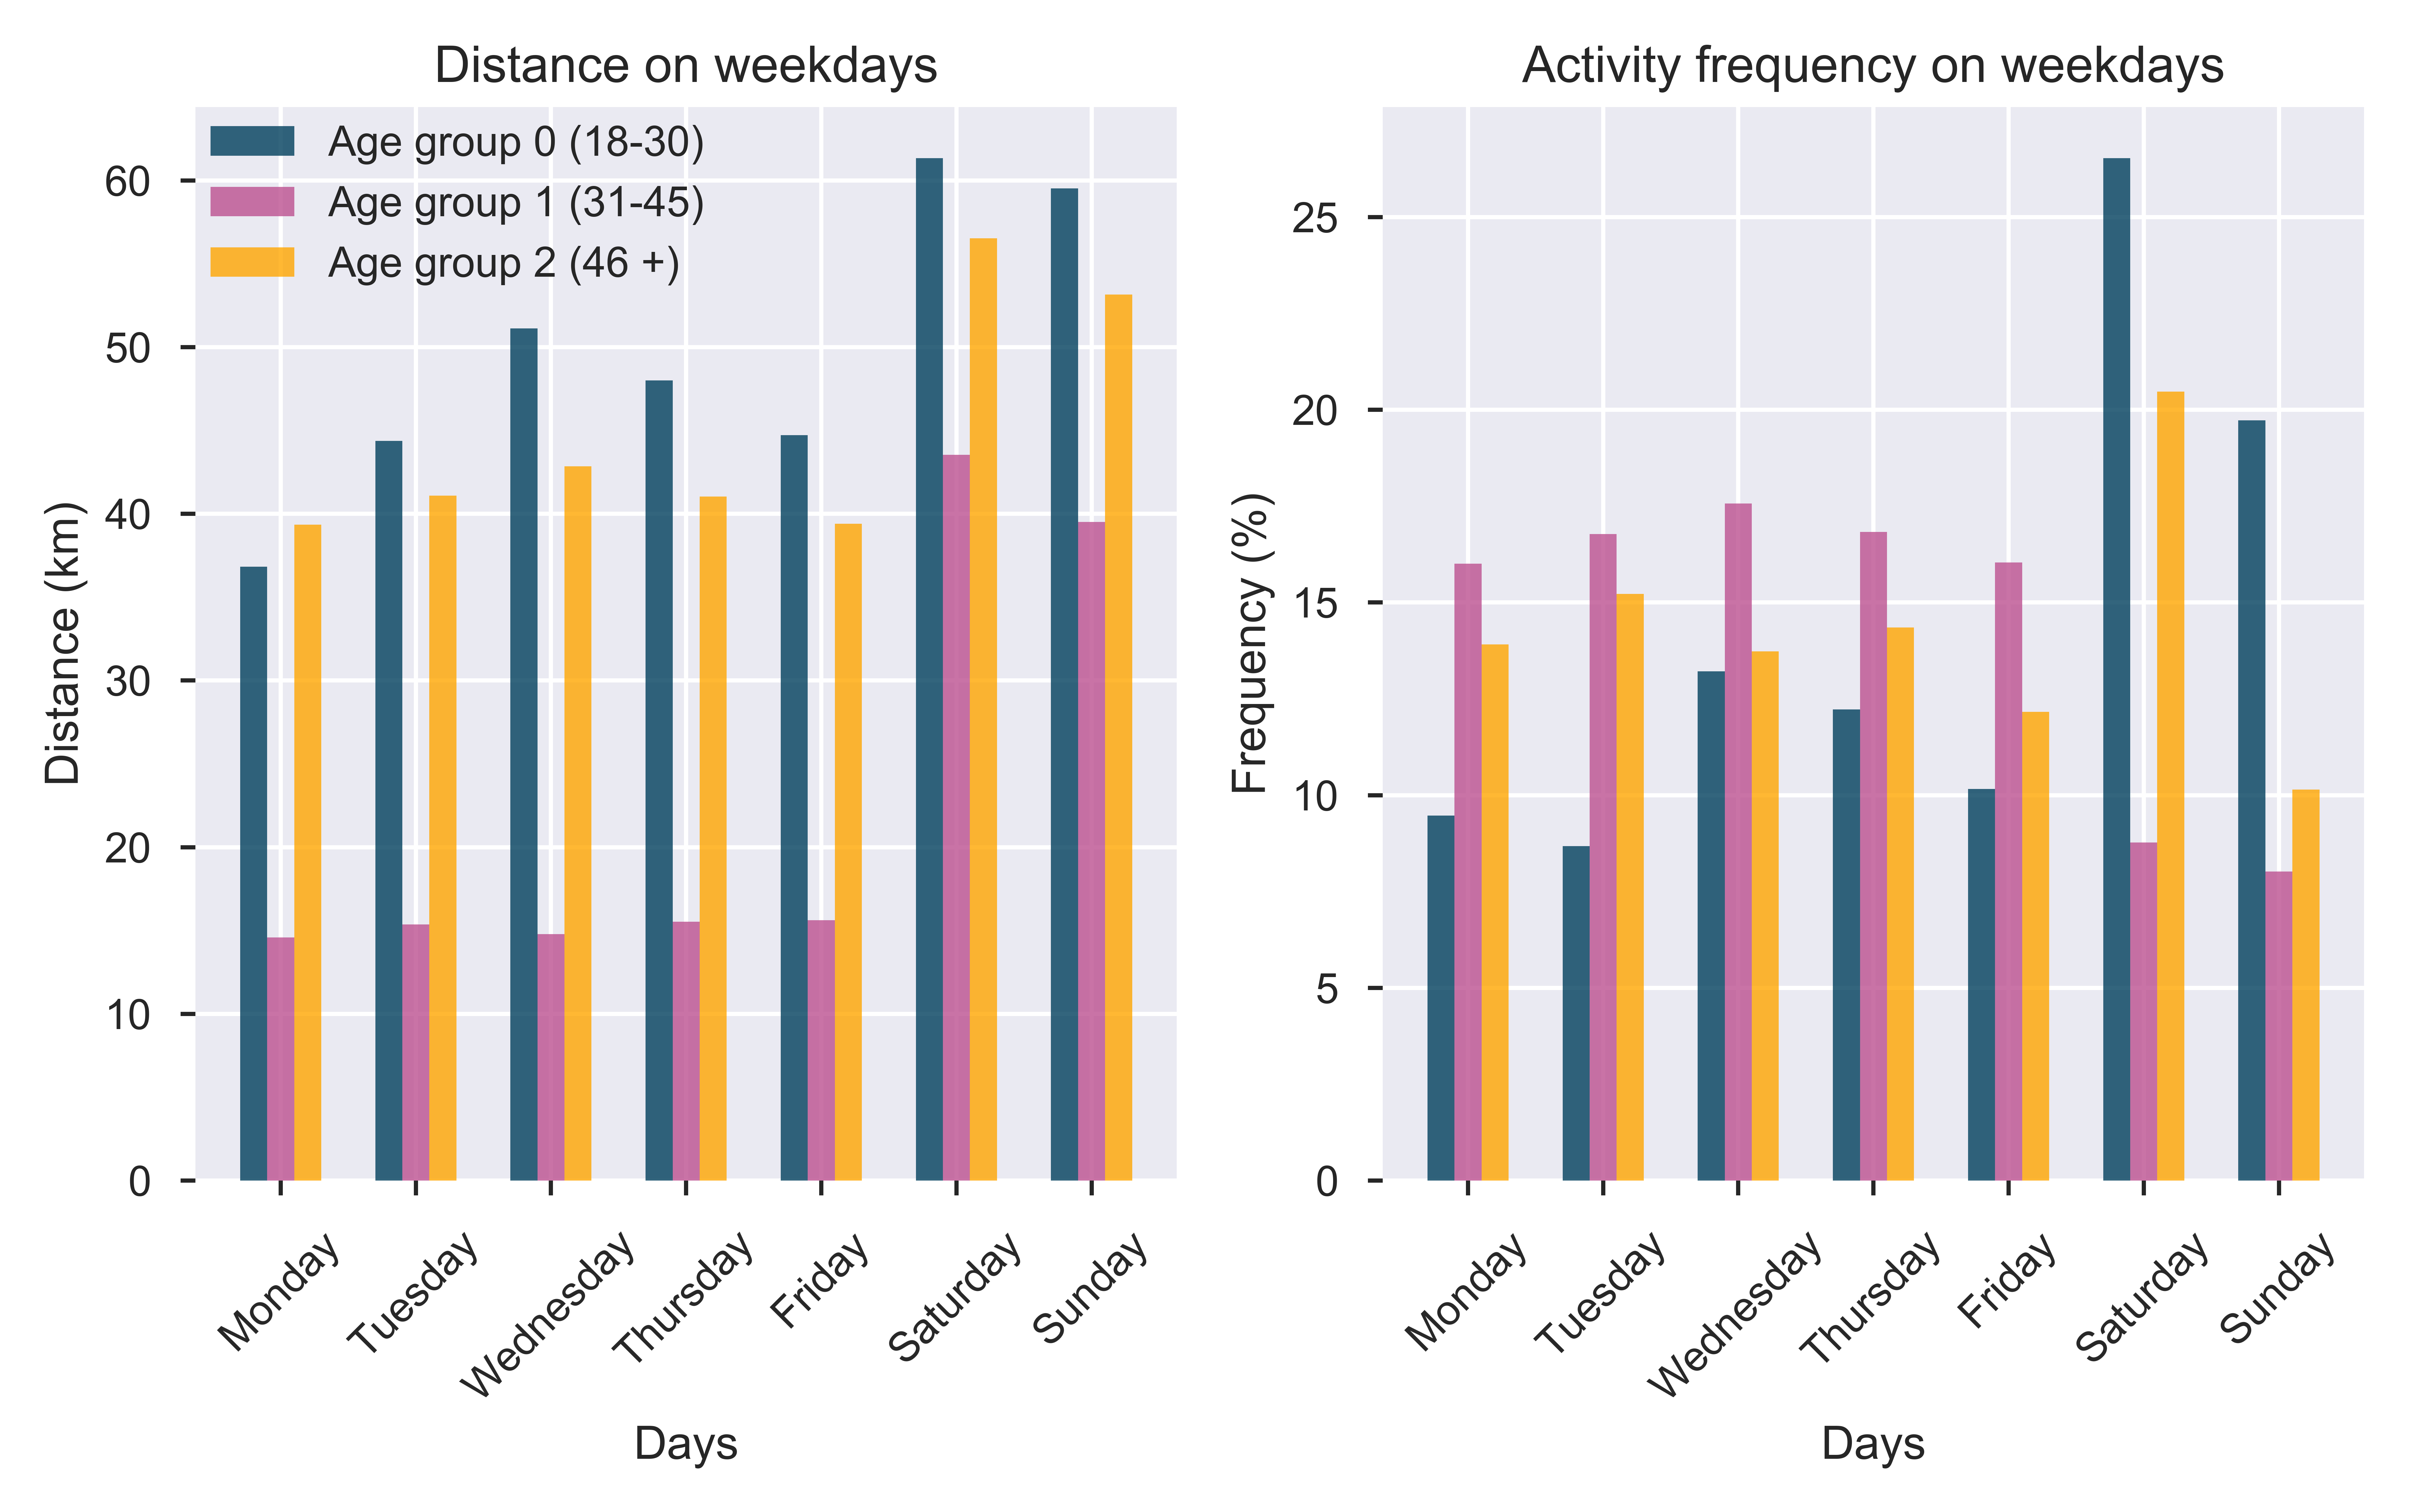
\includegraphics[width=\linewidth]{kepek/FrequencyAndDistanceOnWeekDays.png}
	\caption{Átlagos távolság és útvonal gyakoriság a hét napjain}
	\label{fig:distanceAndFrequencyByWeekdays}
\end{figure}

A \myref{fig:distanceAndFrequencyByWeekdays} ábrán két grafikon jellemzi az útvonalak eloszlását a hét napjai szerint. A bal oldali gráfon az átlagosan megtett távolságot, a jobb oldali pedig az útvonalak darabszámának eloszlását jelzi, korcsoportok szerint lebontva.


Szöveg a fenti képről....

Blablabla

Még mindig.....


\begin{figure}[!h]
	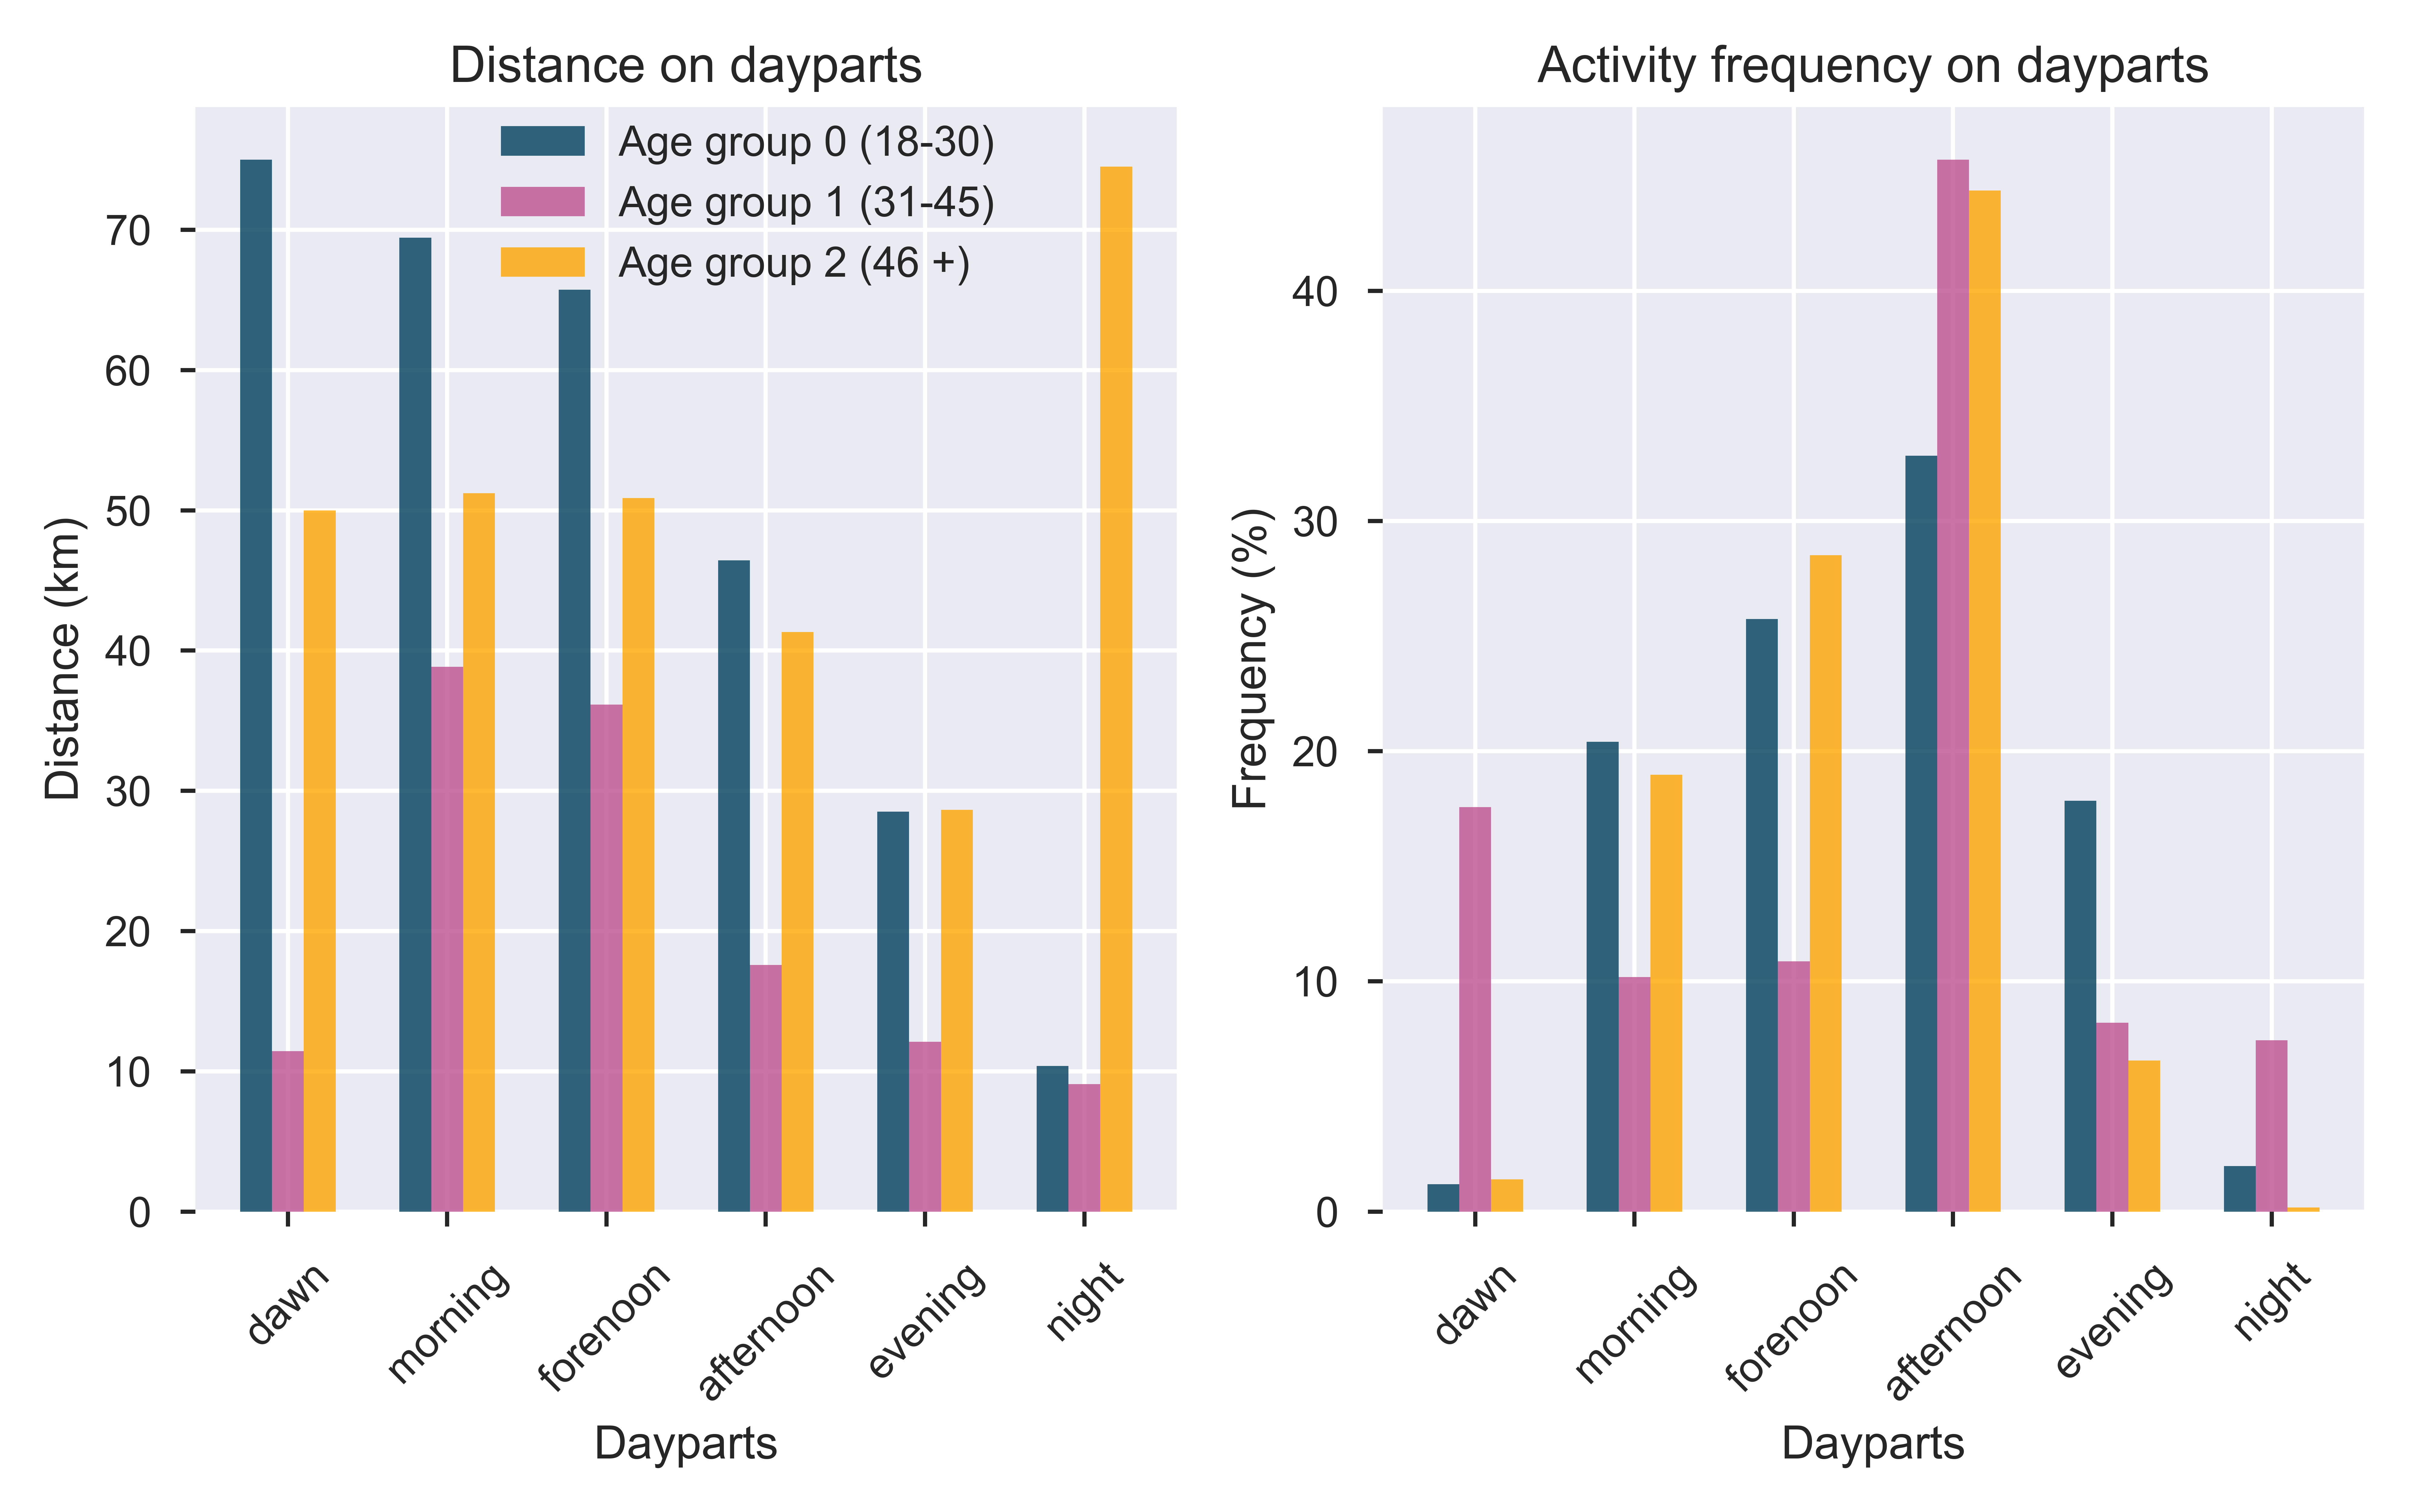
\includegraphics[width=\linewidth]{kepek/FrequencyAndDistanceOnDayparts.png}
	\caption{Átlagos távolság és útvonal gyakoriság napszakok szerint}
	\label{fig:distanceAndFrequencyByDayparts}
\end{figure}








\SubSection{További adat feldolgozás}

\subsubsection{One-hot encoding}
A kiugró értékek kezelése és a adathalmaz összefüggéseinek vizsgálata után a következő lépés a one-hot encoding. Az eljárás lényege hogy egy kategória alapú jellemzőt több (a kategóriák számának megfelelő) oszlopra bont szét, ahol az egyes oszlopokban, jellemzőkben 1-es szerepel amennyiben az adatsor abba az adott kategóriába sorolható, 0 egyébként. Ennek az előnye hogy kiküszöböli a kategóriák sorszámmal történő jelzésének távolságát. Például egy korcsoportot tároló jellemző esetén nem biztos hogy helyes feltételezni hogy a 0. és a 2. kategória (csoport) között 2 távolság van. A one hot encoding természetesen folytonos változók esetén nem értelmezhető és kategoriális jellemzőkre sem mindig érdemes alkalmazni.

A szakdolgozathoz használt adathalmaz esetén 3+1 jellemző kerül one-hot encode-olásra: age\_group (korcsoport), workout\_tpye, start\_date\_local és a training.\\[6pt]

\textbf{age\_group:} a sportoló korcsoportját jelzi, értékei egy három elemű halmazból kerülhetnek ki: \{0, 1, 2\} ahol 0 a [18, 30], 1 a [31, 45], 2 pedig a [46, $+\infty$) korcsoportokba való tartozást jelenti. One-hot encoding során az eredeti jellemzőből 3 oszlop készül, végül az eredeti törlésre kerül az adathalmazból.
\begin{programreszlet}
Python parancsok részletezése
\begin{python}
ageOneHot = pandas.get_dummies(rawData['age_group'], prefix='age')
rawData.drop(columns=['age_group'], inplace=True)
rawData = rawData.join(ageOneHot)
\end{python}
\end{programreszlet}
A kódban megadott prefix paraméter segítségével az új jellemzők nevei: age\_0.0, age\_1.0, age\_2.0\\[6pt]


\textbf{workout\_tpye:} 

\begin{programreszlet}
	\TODO szöveg
\begin{python}
workoutTypeOneHot = pandas.get_dummies(rawData['workout_type'],
				       prefix='workout_type')
rawData.drop(columns='workout_type', inplace=True)
rawData = rawData.join(workoutTypeOneHot)
\end{python}
\end{programreszlet}


\textbf{start\_date\_local:} a jellemző az aktivitás kezdeti idejét tárolja, a sportoló saját időzónája szerint, ÉÉÉÉ-MM-DD HH:MM:SS formátumban. Dátum mezők azonban nem értelmezhetőek gépi tanulási algoritmusokkal így a jellemző átalakítása szükségszerű volt. A dátumból alapvetően 2 féle új jellemző kerül kinyerésre, majd ezek külön kerülnek one-hot encode-olásra

\begin{programreszlet}
Az aktivitás kezdetének dátumából kinyerhető hogy a hét melyik napján történt az aktivitás. Ezen információ kinyerését és one-hot encode-olását az alábbi kód végzi
\begin{python}
rawData['day_of_week'] = rawData['start_date_local'].dt.day_name()
weekDayOneHot = pandas.get_dummies(rawData['day_of_week'], 
				   prefix='weekday')
rawData.drop(columns=['day_of_week'], inplace=True)
rawData = rawData.join(weekDayOneHot)
\end{python}		
\end{programreszlet}

\begin{programreszlet}
Az aktivitás kezdetének időpontjából kinyerhető hogy melyik napszakban kezdődött az aktivitás. Ezen információ kinyerését és one-hot encode-olását az alábbi kód végzi
\begin{python}
rawData['daypart'] = rawData['start_date_local'].apply(lambda row: 
						 timeToPartOfDay(row))
dayPartOneHot = pandas.get_dummies(rawData['daypart'], prefix='daypart')
rawData.drop(columns=['daypart'], inplace=True)
rawData = rawData.join(dayPartOneHot)
\end{python}	

Ahol a timeToPartOfDay függvény a start\_date\_local jellemző minden adattagjára külön hívódik meg. Ez a függvény szubjektíven oszt fel egy napot hat napszakra \myaref{fig:daypartsClock} ábra szerint

\end{programreszlet}

\begin{figure}[!h]
	\centering
	\begin{tikzpicture}[line cap=rect,line width=3pt]
	\filldraw[fill=chart5, draw=chart5, line width=1pt] (0,0)-- +(45:2) arc (45:0:2); %hajnal
	\filldraw[fill=chart0, draw=chart0, line width=1pt] (0,0)-- +(120:2) arc (120:45:2); %éjszaka
	\filldraw[fill=chart1, draw=chart1, line width=1pt] (0,0)-- +(180:2) arc (180:120:2); %este
	\filldraw[fill=chart2, draw=chart2, line width=1pt] (0,0)-- +(270:2) arc (270:180:2); %délután
	\filldraw[fill=chart3, draw=chart3, line width=1pt] (0,0)-- +(315:2) arc (315:270:2); %délelőtt
	\filldraw[fill=chart4, draw=chart4, line width=1pt] (0,0)-- +(360:2) arc (360:315:2); %reggel
	
	\node[font=\small] at (90:2.36cm) {\textsf{Éjszaka}};
	\node[font=\small] at (20:2.7cm) {\textsf{Hajnal}};
	\node[font=\small] at (340:2.7cm) {\textsf{Reggel}};
	\node[font=\small] at (305:2.6cm) {\textsf{Délelőtt}};
	\node[font=\small] at (215:2.7cm) {\textsf{Délután}};
	\node[font=\small] at (155:2.6cm) {\textsf{Este}};
	
	\draw (0,0) circle [radius=2cm];
	
	\foreach \angle [count=\xi] in {75,60,...,-270}
	{
		\draw[line width=1pt] (\angle:1.8cm) -- (\angle:2cm);
		%\node[font=\small] at (\angle:1.36cm) {\textsf{\xi}};
	}
	\foreach \angle [count=\xi] in {0,45,90,135,180,225,270,315}
	{
		\draw[line width=2pt] (\angle:1.6cm) -- (\angle:2cm);
	}
	\draw (0,0) -- (120:0.8cm);
	\draw (0,0) -- (90:1cm);
	\node[font=\small] at (0:1.36cm) {\textsf{6}};
	\node[font=\small] at (45:1.36cm) {\textsf{3}};
	\node[font=\small] at (90:1.36cm) {\textsf{0}};
	\node[font=\small] at (135:1.30cm) {\textsf{21}};
	\node[font=\small] at (180:1.36cm) {\textsf{18}};
	\node[font=\small] at (225:1.36cm) {\textsf{15}};
	\node[font=\small] at (270:1.36cm) {\textsf{12}};
	\node[font=\small] at (315:1.36cm) {\textsf{9}};
	
	
	%\filldraw[line color=gray!40 ] -- +(45:2) arc (45:-45:2);
	\end{tikzpicture}
	\caption{Napszakok kialakítása.}
	\label{fig:daypartsClock}
\end{figure}

\textbf{trainer: } a trainer jellemző Igaz / Hamis értékekkel jelzi hogy egy adott aktivitás traineren, azaz gépen történt e, nem pedig tényleges kerékpáron. Ennek a jellemzőnek az átalakítása nem igazi one-hot encoding, inkább csak az Igaz / Hamis értékek átalakítása 1 / 0 értékekre.  


Az adattisztítás összes lépése után az adathalmaz szerkezete lényegesen megváltozik, új jellemzőket tartalmaz (one-hot encoding) valamint az eddigi jellemzők sok esetben más intervallumokba esnek (kiugró értékek kezelése).

Jellemzők:
\begin{itemize}
	\item average\_speed: átlagsebesség az útvonal során (méter / másodperc)
	\item distance: összesen megtett távolság (méter)
	\item elapsed\_time: összesen eltelt idő (másodperc)
	\item elev\_high: útvonal legmagasabb pontja (méter)
	\item elev\_low: útvonal legalacsonyabb pontja (méter)
	\item hashed\_id: sportoló hashelt azonosítója
	\item max\_speed: legnagyobb elért sebesség (méter / másodperc)
	\item moving\_time: mozgással töltött idő (másodperc)
	\item total\_elevation\_gain: összesen megtett emelkedés (méter)
	\item age\_0.0: 0. korcsoportba való tartozást jelöli (bináris)
	\item age\_1.0: 1. korcsoportba való tartozást jelöli (bináris)
	\item age\_2.0: 2. korcsoportba való tartozást jelöli (bináris)
	\item trainer\_onehot: útvonal megtétele gépen történt e (bináris)
	\item workout\_type\_0.0: 0 típusú útvonal (bináris)
	\item workout\_type\_4.0: 4 típusú útvonal (bináris)
	\item workout\_type\_10.0: 10 típusú útvonal (bináris)
	\item workout\_type\_11.0: 11 típusú útvonal (bináris)
	\item workout\_type\_12.0: 12 típusú útvonal (bináris)
	\item weekday\_Monday: hétfői aktivitás (bináris)
	\item weekday\_Tuesday: keddi aktivitás (bináris)
	\item weekday\_Wednesday: szerdai aktivitás (bináris)
	\item weekday\_Thursday: csütörtöki aktivitás (bináris)
	\item weekday\_Friday: pénteki aktivitás (bináris)
	\item weekday\_Saturday: szombati aktivitás (bináris)
	\item weekday\_Sunday: vasárnapi aktivitás (bináris)
	\item daypart\_dawn: hajnali indulás (bináris)
	\item daypart\_morning: reggeli indulás (bináris)
	\item daypart\_forenoon: délelőtti indulás (bináris)
	\item daypart\_afternoon: délutáni indulás (bináris)
	\item daypart\_evening: esti indulás (bináris)
	\item daypart\_night: éjszakai indulás (bináris)
\end{itemize}


Az adathalmaz ezen a ponton mentésre kerül a későbbi felhasználás megkönnyítésének céljából. A tisztított adatot a \textit{data\_advanced\_\{date\}.csv} fájl tartalmazza.


A tisztított adathalmaz numerikus oszlopainak összefoglalása a \myref{tab:cleanDataDescription} táblázatban található.

% Please add the following required packages to your document preamble:
% \usepackage{graphicx}
% Please add the following required packages to your document preamble:
% \usepackage{graphicx}
\begin{table}[!h]
	\resizebox{\textwidth}{!}{%
		\begin{tabular}{l|l|l|l|l|l|l|l|l|}
			\cline{2-9}
			& \textbf{count} & \textbf{mean} & \textbf{std} & \textbf{min} & \textbf{0.25} & \textbf{0.50} & \textbf{0.75} & \textbf{max} \\ \hline
			\multicolumn{1}{|l|}{\textbf{average\_speed}}                                                    & 9603           & 5.76          & 1.22         & 2.03         & 4.99          & 5.74          & 6.46          & 12.48        \\ \hline
			\multicolumn{1}{|l|}{\textbf{distance}}                                                          & 9603           & 26140.85      & 29199.25     & 161.0        & 7451.3        & 13702.2       & 34599.1       & 436806.0     \\ \hline
			\multicolumn{1}{|l|}{\textbf{elapsed\_time}}                                                     & 9603           & 5817.39       & 19632.69     & 61.0         & 1645.0        & 2998.0        & 7338.5        & 1806211.0    \\ \hline
			\multicolumn{1}{|l|}{\textbf{elev\_high}}                                                        & 9603           & 270.73        & 166.61       & -71.2        & 162.3         & 229.4         & 290.5         & 956.0        \\ \hline
			\multicolumn{1}{|l|}{\textbf{elev\_low}}                                                         & 9603           & 129.92        & 47.88        & -134.4       & 103.2         & 130.2         & 148.3         & 809.6        \\ \hline
			\multicolumn{1}{|l|}{\textbf{max\_speed}}                                                        & 9603           & 12.22         & 3.24         & 2.3          & 9.7           & 11.6          & 14.4          & 22.0         \\ \hline
			\multicolumn{1}{|l|}{\textbf{moving\_time}}                                                      & 9603           & 4509.68       & 4948.21      & 61.0         & 1440.0        & 2415.0        & 6099.0        & 90983.0      \\ \hline
			\multicolumn{1}{|l|}{\textbf{\begin{tabular}[c]{@{}l@{}}total\_elevation\\ \_gain\end{tabular}}} & 9603           & 274.47        & 410.03       & 0.0          & 29.8          & 87.0          & 359.45        & 3896.8       \\ \hline
		\end{tabular}%
	}
\caption{Tisztított adathalmaz numerikus oszlopai}
\label{tab:cleanDataDescription}
\end{table}


% ADATTISZTITAS VEGE


% ML KEZDETE

\Section{Gépi tanulás}

Az adathalmaz egy aktivitásra tekintve két különböző időtartamot különböztet meg: a mozgással töltött (moving\_time) és az összesen eltelt (elapsed\_time) időt, mindkettőt másodpercben mérve. A szakdolgozat során ennek a két időtartamnak a várható értékének a meghatározása az egyik cél gépi tanulási algoritmusokkal valamint ezen algoritmusoknak az összehasonlítása. Ennek a feladatnak a megoldásához a  \myref{subsec:regression} alfejezetben kifejtett regressziók adnak alapot.

A kétféle időtartam alapvetően külön kezelve, egyenként kerül becslésre, erre kivételt csak a \myref{ssec:mlpregressor} pontban részletezett MLPRegressor fog jelenteni.

%% MOVING_TIME
\SubSection{Mozgási idő számítása}

A tisztított adathalmaz beolvasása után szükséges kialakítani az $X$ és $y$ halmazokat amelyek a \TODO adatokat tartalmazzák. Az $y$ fogja tartalmazni a moving\_time jellemzőt míg $X$ minden mást ami alapján $y$ megbecsülhető. 

A regressziók során nagyon fontos az adathalmaz skálázása, egy intervallumra hozása. Ennek fontossága akkor mutatkozik meg igazán mikor a különböző jellemzők nagyon eltérő intervallumokba esnek, például az average\_speed 2.03 és 12.478 értékek között mozog míg a distance 161 és 436806 között. Ezért a gépi tanulás során gyakran alkalmazott eljárás az adathalmaz normalizálása vagy standardizálása amely az összes jellemzőt egy szűk intervallumra vetíti le. A standardizálás elvégzésére a szakdolgozat során a scikit-learn csomag által biztosított StandardScaler függvény szolgál.

\begin{programreszlet}   
Adathalmaz standardizálása

\begin{python}
from sklearn.preprocessing import StandardScaler
X = dataset.copy()

names = X.columns
scaler = StandardScaler()

scaledData = scaler.fit_transform(X)
scaledData = pandas.DataFrame(scaledData, columns=names)
\end{python}
\label{prog:movingStandard}
\end{programreszlet}

\begin{programreszlet} A túltanulás elkerülése érdekében a tanító és cél adathalmazokat szét kell osztani tanító és tesztelő részekre. A regressziós modellek csak a tanító (train) adatokon fognak tanulni, ellenőrzésre, pontosság meghatározására pedig a teszt (test) adatok szolgálnak. A tanító és teszt adathalmazok kialakítására a scikit-learn csomag álltal biztosított train\_test\_split függvény szolgál.
\begin{python}
from sklearn.model_selection import train_test_split
	
scaledY = scaledData['moving_time']
scaledData.drop(columns=['moving_time','elapsed_time'], inplace=True)

trainX, testX, trainy, testy = train_test_split(scaledData, scaledY, 
						random_state=42)
\end{python}
\label{prog:movingTrainTestSplit}
\end{programreszlet}

A \myref{prog:movingStandard} és a \myref{prog:movingTrainTestSplit} program részletek segítségével két különböző adathalmaz kerül kialakításra. Az első esetében az $X$ halmaz a moving\_time és az elapsed\_time oszlopok kivételével minden jellemzőt tartalmaz míg a második esetben az $X$ halmazban csupán a következő jellemzők találhatóak meg:  age\_0.0, age\_1.0, age\_2.0, distance, elev\_high, elev\_low, hashed\_id, total\_elevation\_gain, trainer\_onehot. Az $y$ halmaz mindkét esetben a moving\_time jellemzőt tartalmazza. Mindkét adathalmaz felosztásra került tanító és tesztelő részhalmazokra a train\_test\_split függvény segítségével. A részhalmazok prefixei: all és reduced.

\subsubsection{Ridge regresszió:} ez az algoritmus 2 fő paraméterrel finomhangolható: $\alpha \geq 0 $ és solver $\in$ \{auto, svd, cholesky, lsqr, sparce\_cg, sag, saga\}. Az $\alpha$ paraméter a regularizáció mértékét befolyásolja a különböző solver-ek pedig a számítási rutint befolyásolják (lsd.: dokumentáció). Az algoritmus optimalizálása során $\alpha \in$ \{0.0001, 0.0003, 0.001, 0.003, 0.01, 0.1, 0.3, 0.35, 0.6\} értékek kerültek figyelembe vételre.

% \TODO kifejtés. A moving\_time esetén a standardizált adathalmazra a legoptimálisabb (legnagyobb pontosságot eredményező paraméterek) a $\alpha = 0.003$ solver : saga. Ezeknek az alkalmazása esetén, a modellt a trainX és trainy adathalmazokon tanítva a pontosság 96.251\% (a teszt adatokon). A modell nem tanul túl, mivel a teszt adatokon (amiket a modell tanulás során nem ismer) nagy pontosság jellemzi a regressziót.

\subsubsection{Lasso regresszió:} a modell finomhangolása elsősorban az $\alpha \geq 0$ paraméter változtatásával történik. A scikit-learn implementáció lehetőséget ad egyéb opciók beállítására azonban ezek nem befolyásolják nagyban a modell működését így használatuk mellőzésre kerül a szakdolgozat során. Az optimalizálás során $\alpha \in$ \{0.0001, 0.0003, 0.001, 0.003, 0.01, 0.1, 0.3, 0.35, 0.6\} értékek kerültek figyelembe vételre.
%$\alpha = 0.0001$, pontosság: 96.246\%


\subsubsection{Random Forest regresszió:} ez a döntési fákon alapuló eljárás lényegesen mélyebben személyre szabható a paraméterei révén mint a Ridge és a Lasso regresszió. Optimalizálása során a következő paraméterek kerültek felhasználásra:
\begin{itemize}
	\item n\_estimators$\in$ \{200, 500, 1000\}: fák száma
	\item max\_depth $\in$ \{NaN, 10, 50, 100\}: fák maximum mélysége
	\item max\_features $\in$ \{auto, sqrt\}: a legjobb felosztás megtalálásához felhasználandó jellemzők darabszáma
	\item min\_samples\_leaf $\in$ \{1, 2, 4\}: egy levél legalább hány mintát tartalmazzon
	\item min\_samples\_split $\in$ \{2, 5, 10\}: csomópontok felosztásához szükséges mintaszám
	\item bootstrap $\in$ \{True, False\}: teljes adathalmaz vagy részhalmazok felhasználásával kerüljenek kialakításra az egyes fák
\end{itemize}
A Random Forest egyéb paraméterei is befolyásolhatják a tanulás eredményességét, a becslések pontosságát. 


\subsubsection{Eredmények}

Ridge és Lasso regresszió
\begin{table}[!h]
	\centering
	\begin{tabular}{|l|r|r|r|r|c|}
		\hline
		\textbf{Modell} & \textbf{X} & \textbf{y}   & \multicolumn{1}{l|}{\textbf{Pontosság}} & \textbf{$\boldsymbol\alpha$} & \multicolumn{1}{l|}{\textbf{Solver}} \\ \hline
		\textbf{Ridge}  & all        & moving\_time & 0.962492                                & 0.01              & saga                                 \\ \hline
		\textbf{Ridge}  & reduced    & moving\_time & 0.938656                                & 0.01              & saga                                 \\ \hline
		\textbf{Lasso}  & all        & moving\_time & 0.962469                                & 0.0001            & --                                   \\ \hline
		\textbf{Lasso}  & reduced    & moving\_time & 0.938630                                & 0.0001            & --                                   \\ \hline
	\end{tabular}
\caption{Ridge és Lasso eredmények moving\_time jellemző becslésére}
\end{table}

összegző szöveg Ridge és Lasso eredményekről

Random Forest regresszió


szöveg
\begin{table}[!h]
	\centering
	\begin{tabular}{|l|r|r|}
		\hline
		\textbf{Modell}              & \multicolumn{1}{l|}{\textbf{Random Forest}} & \multicolumn{1}{l|}{\textbf{Random Forest}} \\ \hline
		\textbf{X}                   & all                                         & reduced                                     \\ \hline
		\textbf{y}                   & moving\_time                                & moving\_time                                \\ \hline
		\textbf{Score}               & 0.957091                                    & 0.923862                                    \\ \hline
		\textbf{n\_estimators}       & 200                                         & 200                                         \\ \hline
		\textbf{max\_depth}          & 50                                          & 50                                          \\ \hline
		\textbf{max\_features}       & auto                                        & auto                                        \\ \hline
		\textbf{min\_samples\_leaf}  & 2                                           & 2                                           \\ \hline
		\textbf{min\_samples\_split} & 2                                           & 2                                           \\ \hline
		\textbf{bootstrap}           & True                                        & True                                        \\ \hline
	\end{tabular}
\caption{Random Forest regresszió eredmények moving\_time jellemző becslésére}
\end{table}



\subsubsection{Moving\_time összefoglalás}

%% MOVING_TIME END


%% ELAPSED_TIME
\SubSection{Eltelt idő számítása}

A tisztított adathalmaz beolvasása után szükséges kialakítani az $X$ és $y$ halmazokat amelyek a \TODO adatokat tartalmazzák. Az $y$ fogja tartalmazni a elapsed\_time jellemzőt míg $X$ minden mást ami alapján $y$ megbecsülhető. 

A regressziók során nagyon fontos az adathalmaz skálázása, egy intervallumra hozása. Ennek fontossága akkor mutatkozik meg igazán mikor a különböző jellemzők nagyon eltérő intervallumokba esnek, például az average\_speed 2.03 és 12.478 értékek között mozog míg a distance 161 és 436806 között. Ezért a gépi tanulás során gyakran alkalmazott eljárás az adathalmaz normalizálása vagy standardizálása amely az összes jellemzőt egy szűk intervallumra vetíti le. A standardizálás elvégzésére a szakdolgozat során a scikit-learn csomag által biztosított StandardScaler függvény szolgál.

\begin{programreszlet}   
	Adathalmaz standardizálása	
\begin{python}
from sklearn.preprocessing import StandardScaler
X = dataset.copy()
		
names = X.columns
scaler = StandardScaler()
		
scaledData = scaler.fit_transform(X)
scaledData = pandas.DataFrame(scaledData, columns=names)
\end{python}
\label{prog:elapsedStandard}
\end{programreszlet}

\begin{programreszlet} A túltanulás elkerülése érdekében a tanító és cél adathalmazokat szét kell osztani tanító és tesztelő részekre. A regressziós modellek csak a tanító (train) adatokon fognak tanulni, ellenőrzésre, pontosság meghatározására pedig a teszt (test) adatok szolgálnak. A tanító és teszt adathalmazok kialakítására a scikit-learn csomag álltal biztosított train\_test\_split függvény szolgál.
\begin{python}
from sklearn.model_selection import train_test_split
		
scaledY = scaledData['elapsed_time']
scaledData.drop(columns=['elapsed_time'], inplace=True)
		
trainX, testX, trainy, testy = train_test_split(scaledData, scaledY, 
						random_state=42)
\end{python}
\label{prog:elapsedTrainTestSplit}
\end{programreszlet}

A \myref{prog:elapsedStandard} és a \myref{prog:elapsedTrainTestSplit} program részletek segítségével 7 különböző adathalmaz kerül kialakításra. A cél mindig az elapsed\_time jellemző becslése amelyet egyik X sem tartalmaz
\begin{itemize}
	\item \textbf{all:} X minden jellemzőt tartalmaz (elapsed\_time kivételével)
	\item \textbf{reduced:} X csökkentett számú jellemzőt tartalmaz, név szerint a következőket: age\_0.0, age\_1.0, age\_2.0, distance, elev\_high, elev\_low, hashed\_id, total\_elevation\_gain, moving\_time, trainer\_onehot
	\item \textbf{ageNull:} X és y is csak a 0 korcsoportba (18-30) tartozó sportolók adatait tartalmazza 
	\item \textbf{ageOne:} X és y is csak az 1 korcsoportba (31-45) tartozó sportolók adatait tartalmazza
	\item \textbf{ageTwo:} X és y is csak a 2 korcsoportba (46+) tartozó sportolók adatait tartalmazza
	\item \textbf{distanceSmall:} X csak olyan útvonalakat tartalmaz ahol a távolság kisebb mint 50 km
	\item \textbf{distanceBig:} X csak olyan útvonalakat tartalmaz ahol a távolság nagyobb mint 50 km
	
\end{itemize}



\subsubsection{Eredmények}

Ridge és Lasso regresszió
% Please add the following required packages to your document preamble:
% \usepackage{booktabs}
\begin{table}[h!]
	\centering
	\begin{tabular}{|r|c|r|r|c|}
			\hline
			\textbf{X}    & \textbf{Modell} & \multicolumn{1}{l|}{\textbf{Pontosság}} & \multicolumn{1}{l|}{\textbf{$\alpha$}} & \textbf{Solver} \\ \hline
			all           & Ridge           & 0.722601                                & 0.35                                   & lsqr            \\ \hline
			all           & Lasso           & 0.733696                                & 0.01                                   & --              \\ \hline
			reduced       & Ridge           & 0.741402                                & 0.6                                    & saga            \\ \hline
			reduced       & Lasso           & 0.742481                                & 0.001                                  & --              \\ \hline
			ageNull       & Ridge           & 0.922961                                & 0.003                                  & saga            \\ \hline
			ageNull       & Lasso           & 0.923146                                & 0.003                                  & --              \\ \hline
			ageOne        & Ridge           & 0.756610                                & 0.0                                    & auto            \\ \hline
			ageOne        & Lasso           & 0.774819                                & 0.01                                   & --              \\ \hline
			ageTwo        & Ridge           & 0.914806                                & 0.6                                    & saga            \\ \hline
			ageTwo        & Lasso           & 0.917202                                & 0.003                                  & --              \\ \hline
			distanceSmall & Ridge           & 0.325245                                & 0.6                                    & sag             \\ \hline
			distanceSmall & Lasso           & 0.384225                                & 0.01                                   & --              \\ \hline
			distanceBig   & Ridge           & 0.823487                                & 0.6                                    & saga            \\ \hline
			distanceBig   & Lasso           & 0.908215                                & 0.1                                    & --              \\ \hline
	\end{tabular}
\caption{Ridge és Lasso eredmények elapsed\_time becsléséhez}
\end{table}

összegző szöveg Ridge és Lasso eredményekről

Random Forest regresszió


szöveg
\begin{table}[!h]
	\centering
	
	\caption{Random Forest regresszió eredmények elapsed\_time jellemző becslésére}
\end{table}



\subsubsection{Elapsed\_time összefoglalás}
%\Section{Programkód}
